% IEEEAerospace2012.cls requires the following packages: times, rawfonts, oldfont, geometry
\documentclass[twocolumn,letterpaper]{IEEEAerospaceCLS}  % only supports two-column, letterpaper format

% The next line gives some packages you may find useful for your paper--these are not required though.
%\usepackage[]{graphicx,float,latexsym,amssymb,amsfonts,amsmath,amstext,times,psfig}
% NOTE: The .cls file is now compatible with amsmath!!!

\usepackage{siunitx}      % Use for scientific notation.
\usepackage{float}        % Use to not have figures placed in random locations.
\usepackage[]{graphicx}   % We use this package in this document.
\usepackage[font=footnotesize,labelfont=bf,textfont=bf]{caption}
\usepackage{subcaption}   % neue subfigure-Umgebung %% should probably not be used with memoir: generates warning
\usepackage[nolist,nohyperlinks]{acronym} % Use this for acronyms, unlisted.

% URL hyperlinks in References section.
\usepackage{hyperref}

%\hypersetup{
%  colorlinks=true,
%  linkcolor=blue,
%  filecolor=magenta,
%  urlcolor=cyan,
%}

%\urlstyle{same}


% New commands.
\newcommand{\ignore}[1]{}                  % {} empty inside = %% comment.
\newcommand{\refFig}[1]{{Figure}~\ref{#1}} % Command for figure reference.
\newcommand{\refTab}[1]{{Table}~\ref{#1}}  % Command for table reference.

% For block commenting
\newcommand{\comment}[1]{}

% Renew commands.

% Use alpha for footnotes.
\renewcommand\thefootnote{{(\alph{footnote})}} % footnote formatting and colors

% Define common figure sizes for subfigures -> redefined in each environment
\newlength{\subfigureWidth}
\setlength{\subfigureWidth}{0.24\textwidth}
\newlength{\graphicsHeight}
\setlength{\graphicsHeight}{25mm}


\begin{acronym}
  \acro{DFKI}{German Research Center for Artificial Intelligence}
  \acro{EOL}{End of Life}
  \acro{IL}{InnerLeg}
  \acro{MRS}{Multi-Robot System}
  \acro{OL}{OuterLeg}
  \acro{PLI}{Payload Item}
  \acro{RA}{Robotic Arm}
  \acro{RIC}{Robotics Innovation Center}
  \acro{SA}{Solar Array}
  %\acrodefplural{SA}[SAs]{Solar Arrays}
  \acro{TRL}{Technology Readiness Level}
  \acro{WD}{WheelDrive}
  \acro{WS}{WheelSteering}
\end{acronym}

\begin{document}
\title{Using a Rover's Active Suspension System as a 2-Axis Solar Tracker Mechanism}

% Alternative titles:
%   1. Daily Solar Array Reconfiguration with the SherpaTT Rover Active Suspension System for Long Traverses
%   2. Extending Rover Traverse Coverage with the SherpaTT Active Suspension System for Daily Solar Array Reconfiguration
%   3. Using the SherpaTT Active Suspension for Daily Optimization of Solar Array Configuration
%   4. The SherpaTT Rover's Active Suspension System as a Mechanism for Daily Optimization of Solar Array Configuration
%   5. Using the SherpaTT Active Suspension System for Daily Optimization of Rover Solar Array Configuration
%   6. The SherpaTT Rover Active Suspension System as a Mechanism for Daily Solar Array Optimization
%   7. Mars Traverse Distance Gains Using a Rover's Active Suspension System as a 2-Axis Solar Tracker Mechanism
\author{%
Georges L. J. Labrèche\\
Georges.Labreche@gmail.com
\and
Florian Cordes\footnote{DFKI Robotics Innovation Center, Robert-Hooke-Straße 1, 28359 Bremen, Germany.}\\
Florian.Cordes@dfki.de
}

% Extra vertical spacing in table cells.
%{\renewcommand{\arraystretch}{1.5}% for the vertical padding

\maketitle

\thispagestyle{plain}
\pagestyle{plain}


The SherpaTT rover is prepared for further autonomous long distance traverses in terrain akin to the Martian environment. However, it features a fueled power generator which cannot be employed in extra-terrestial scenarios. As the rover is meant to approach a higher technology readiness level, a photovoltaic power subsystem is proposed to guide future design iterations. This paper presents the solar array sizing, design, and integration processes considered for two Martian mission sites: Iani Chaos at \SI{2}{\degree}S and Ismenius Cavus at \SI{34}{\degree}N. An alternative use case for the active suspension system is presented so that the proposed solar arrays may be inclined and oriented into power generating configurations that are more favorable than those achieved with passive suspension rovers. This results in traverse gains of up to \SI{34}{\percent} and \SI{25}{\percent} for clear days at Iani Chaos and Ismenius Cavus, respectively.

The exploration rover SherpaTT has a total mass of approximately \SI{206}{\kilo\gram} and the legs as well as the \ac{RA} weigh about \SI{25}{\kilo\gram} each. The wheeled-leg active suspension system allows the rover to assume different poses with varying inertial moments. The rover is one of many systems comprising a \ac{MRS} developed at the \ac{DFKI}'s \ac{RIC}.

The rover has undergone several field trial campaigns, particularly with a Mars analogue terrain field deployment in Utah, USA, where a logistics chain for sample return was evaluated. The rover's versatility has been demonstrated through a multitude of tasks such as assembling surface deployable payloads and using its \ac{RA} for soil sampling with modular \ac{PLI} sampling devices \cite{Cordes2018b}.

\comment{
\begin{figure}[h]
  \centering
  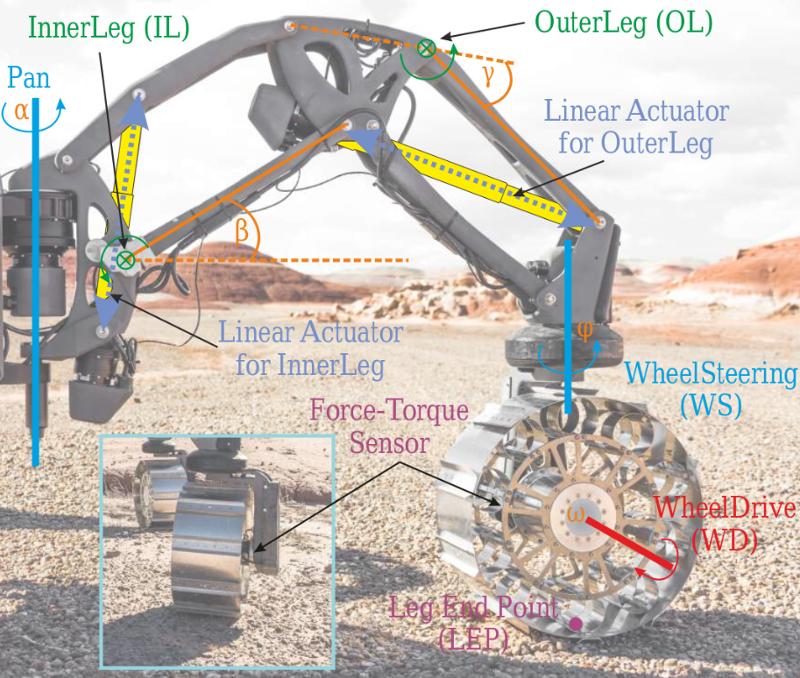
\includegraphics[width=3.2in]{figures/images/sherpatt-actively-articulated-suspension-sytem.png}\\
  \caption{Description of DoF present in SherpaTT’s
suspension system and placement of force-torque sensor}
  \label{fig:sherpatt-actively-articulated-suspension-system}
\end{figure}
}

The active suspension system consists of four wheeled-legs with a total of 20 motors.\comment{Motor distribution across a single leg is shown in \refFig{fig:sherpatt-actively-articulated-suspension-system}.} Each leg is equipped with three suspension motors and two drive motors. The suspension motors are responsible for Pan, \ac{IL}, and \ac{OL} revolute joint rotations whereas the drive motors are responsible for \ac{WS} and \ac{WD}. \comment{A first design iteration of the rover with \ac{SA} for an Ismenius Cavus deployment is shown in \refFig{fig:solar-array-on-ismenius-cavus-chaos}.}

\comment{
\begin{figure}[h]
 \centering
 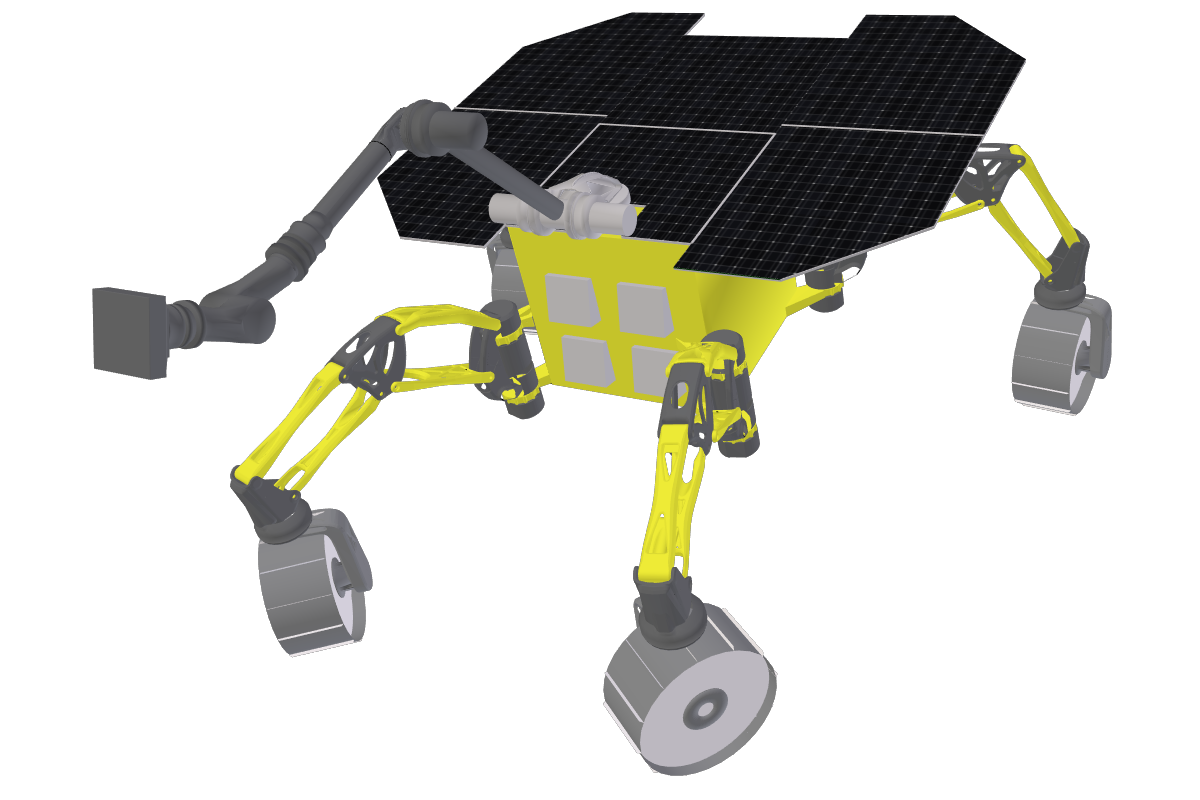
\includegraphics[width=2.8in]{figures/images/ismenius-cavus-10deg-pitch.png}\\
 \caption{Rover with \ac{SA} for Ismenius Cavus deployment.}
 \label{fig:solar-array-on-ismenius-cavus-chaos}
\end{figure}
}

The rover has been deployed in several field experiments where it was put under test within natural and unstructured Mars analogue terrain with respect to general morphology and geology. The rover displayed the ability to cope with natural terrain and to fulfill the task of being an exploration and sampling rover. Further development is required on its electrical power subsystem if it is to operate in long term missions. This paper explores \ac{SA} configurations for the a Mars environment in order to guide future design iterations to navigate the topography of this planetary surface. The constraints imposed from the active suspension system with flexible footprints and varying heights of structural parts of the legs are considered in the design phase.

Initial \ac{SA} sizing requirements are derived from Mars mission sites, Iani Chaos and Ismenius Cavus, that impose energy storage and consumption constraints based on available daily insolations. The design is driven by the use the rover's active suspension system as a 2-axis solar tracking mechanism, enabling daily reconfiguration of the \ac{SA} surface inclination and orientation angles. An alternative use of the wheeled leg system is thus presented for a use case that goes beyond the scenario of negotiating complex terrains such as steep slopes. Specifically, the findings demonstrate traverse and mass reductions gains that are obtained with a suspension system driven inclination and orientation capable \ac{SA} surface when compared to a horizontal configuration.

Past research on active suspension systems are restricted to analyzing benefits with respect to traversing challenging topographies. Studying how this system can be used for other mission planning elements broadens the field of research.

The findings of this paper support using the SherpaTT rover active suspension system as a mechanism for solar panel inclination and orientation under certain \ac{SA} sizing conditions. Combining a maximum attainable \ac{SA} surface inclination angle of \SI{10}{\degree} with optimal daily orientation angles results in appreciable traverse gains when compared to what is obtained from a horizontal surface. However, this is not true for large \ac{SA} areas. Furthermore, the smaller the required solar cell coverage area the greater the gains. In light of this, \ac{SA} sizing for the the worst case daily insolations introduce a hibernation mode solar power draw constraint of \SI{17}{\watt} near the equator at \SI{2}{\degree}S and \SI{15}{\watt} in the northern hemisphere at \SI{34}{\degree}N. \comment{With these power budgets, an average traverse gain of \SI{34}{\percent} is achieved at \SI{2}{\degree}S for a clear day with a $\tau$ factor of 0.4. At \SI{34}{\degree}N, the average gain is \SI{25}{\percent} under the same atmospheric opacity. These gains remain significant on dusty days at \SI{23}{\percent} and \SI{10}{\percent} at respective latitudes with a $\tau$ factor of 1.}

This paper presents an active suspension system use case that goes beyond negotiating complex terrains such as steep slopes or exploring crater environments. The following are a few suggested research topics that expands this idea:

\begin{itemize}
  \item [(1)] Conducting a power budget cost-benefit analysis with respect to the power draws from the suspension systems motors that are required to obtain the sun-facing inclined \ac{SA} surfaces power gains.
  \item [(2)] Achieving higher pitch and rolls angles so that higher \ac{SA} surface inclination angles may be attained.
  \item [(3)] Simulating ground adaption scenarios that preserve a desired \ac{SA} surface position into a fixed plane.
  \item [(4)] Simulating shadowing events on the \ac{SA} and analyzing their affect on power outputs, in particular for shadows caused by the \ac{RA}.
  \item [(5)] Implementing a battery model to simulate battery charge and discharge for a more complete power subsystem simulation.
  \item [(6)] Developing power budgets for onboard instruments to simulate scenarios such as drilling for sample return missions.
  \item [(7)] Proposing SherpaTT \ac{SA} designs for terrestrial and lunar mission scenarios.
  \item [(8)] Exploring other alternative use cases for the rover's active suspension system such as nighttime star tracking for astronomical observations with a mounted telescope.
\end{itemize}

At the time of writing this paper, work is already being done in (5) as part of the ADE (OG10) project for autonomous decision making in very long traverses 
\cite{ADEOG10}.


%%%%%%%%%%%%%%%%%%%%%%%%%%%%%%%%%%%%%%%%%%%%%%%%%%%%%%%%%%%%%%%%%%%%%%%%%%%%%%%%%%%%%%%%%%%%%%%%%%%%%%
\bibliographystyle{IEEEtran}
%\bibliography{IEEEabr,MyBibFile}
\begin{thebibliography}{1}

\bibitem{Cordes2018a}
Cordes, F. Design and Experimental Evaluation of a Hybrid Wheeled-Leg Exploration Rover in the Context of Multi-Robot Systems. PhD thesis, University of Bremen. 2018, \url{https://doi.org/10.13140/RG.2.2.24973.79843}

\bibitem{Cordes2018b}
Cordes, F, Kirchner, F, Babu, A. Design and field testing of a rover with an actively articulated suspension system in a Mars analog terrain. Journal of Field Robotics. 2018; 35: 1149– 1181. \url{https://doi.org/10.1002/rob.21808}

\bibitem{Labreche2020}
Labrèche, G. Exploiting the SherpaTT Rover Active Suspension System to Enable Optimal Solar Array Inclination and Orientation for Long Traverses in a Martian Environment. 2020, \url{http://urn.kb.se/resolve?urn=urn:nbn:se:ltu:diva-78016}

\bibitem{Appelbaum1989}
Appelbaum, J, Flood, D. Solar Radiation on Mars. NASA-TM-102299. 1989, \url{https://ntrs.nasa.gov/?R=19890018252}

\bibitem{Appelbaum1990}
Appelbaum, J, Flood, D. Solar radiation on Mars: Update 1990. NASA-TM-103623. 1990, \url{https://ntrs.nasa.gov/?R=19910005804}

\bibitem{Appelbaum1991}
Appelbaum, J, Flood, D. Solar radiation on Mars: Update 1991. NASA-TM-105216. 1991, \url{https://ntrs.nasa.gov/?R=19910023732}

\bibitem{Appelbaum1993}
Appelbaum, J, Sherman, I, Landis, G. A. Solar radiation on Mars: Stationary photovoltaic array. NASA-TM-106321. 1993, \url{https://ntrs.nasa.gov/?R=19940010257}

\bibitem{Appelbaum1994}
Appelbaum, J, Flood, D, Norambuena, M. Solar radiation on Mars: Tracking photovoltaic array. NASA-TM-106700. 1994, \url{https://ntrs.nasa.gov/?R=19950004977}

\bibitem{Phobos}
DFKI/RIC, Phobos. \url{https://github.com/dfki-ric/phobos}. Accessed on: Jun. 12, 2020.

\bibitem{MARSSim}
DFKI/RIC, MARS - Machina Arte Robotum Simulans. \url{https://robotik.dfki-bremen.de/en/research/softwaretools/mars.html}. Accessed on: Jun. 12, 2020.

\bibitem{ADEOG10}
DFKI/RIC, ADE (OG10) - Autonomous Decision Making in Very Long Traverses. \url{https://robotik.dfki-bremen.de/en/research/projects/ade-og10.html}. Accessed on: Jun. 23, 2020.

\end{thebibliography}

\end{document}
